%%%%%%%%%%%%%%%%%%%%%%%%%%%%%%%%%%%%%%%%%%%%%%%%%%%%%%%%%%%%%%%%%%%%%%%%%%
%% IISc M.Tech (Online) project report
%% AI-Driven Quality Assistance Application for STLC Automation
%%%%%%%%%%%%%%%%%%%%%%%%%%%%%%%%%%%%%%%%%%%%%%%%%%%%%%%%%%%%%%%%%%%%%%%%%%
\documentclass[oneside,12pt]{IIScthesisPSnPDF}

\usepackage{amssymb}
\usepackage{amsmath}
\usepackage{latexsym}
\usepackage{multicol}
\usepackage{booktabs}
\usepackage{multirow}
\usepackage{tabularx}
\usepackage{fancyhdr}
\usepackage[numbers]{natbib}
\usepackage{cleveref}
\usepackage{wrapfig}
\usepackage{float}
\usepackage{algorithm}
\usepackage{algpseudocode}
\usepackage{enumerate}
\usepackage{cancel}
\usepackage{mathrsfs}
\usepackage{color}
\usepackage[compact]{titlesec}
\usepackage{mdwlist}
\usepackage{tikz}
\usepackage{varwidth}
\usepackage{url}
\usepackage{datetime}
\usepackage{pdfpages}
\usepackage{notoccite}
\usepackage{diagbox}
\usepackage{hhline}
\usepackage{subfigure}
\usepackage{etoolbox}
\usetikzlibrary{shapes,arrows,trees,positioning,calc,arrows.meta}

\renewcommand\nomgroup[1]{%
  \item[\bfseries
  \ifstrequal{#1}{A}{Acronyms}{%
  \ifstrequal{#1}{B}{Abbreviations}{%
  \ifstrequal{#1}{S}{Symbols}{}}}%
]}

%This command reserves a whole page for a figure
%Its only argument is the caption
\newcommand{\fullpagefigspace}[2]{
\begin{figure}
\vspace{5.0in}
\caption{#1}
\label{#2}
\end{figure}
}
%            
%
\newcommand{\abs}[1]{$|{#1}|$}
\newcommand{\absq}[1]{$|{#1} |^{2}$}
\newcommand{\tabs}[1]{|{#1}|}
\newcommand{\tabsq}[1]{|{#1}|^2}
\newcommand{\half}{$\frac{1}{2}$}
\newcommand{\nth}{^{\mathrm{th}}}
\newcommand{\prob}[1]{\mathsf{Pr}\left(#1\right)}
\newcommand{\EXP}[1]{\mathsf{E}\!\left(#1\right)}
\newcommand{\D}{\displaystyle}
%%%%%%%%%%%%%%%%%%%%%%%%%%%%%%%%%%%%%%%%%%%%%%%%%%%%%%%%%%%%%%%%%%%%%%%%
%THE FOLLOWING IS FOR MAKING THE CAPTIONS IN SANS SERIF AND PUT A FIGRULE
%%%%%%%%%%%%%%%%%%%%%%%%%%%%%%%%%%%%%%%%%%%%%%%%%%%%%%%%%%%%%%%%%%%%%%%%
%\newcommand{\captionfonts}{\sf}

%\makeatletter  % Allow the use of @ in command names
%\long\def\@makecaption#1#2{%
%  \vskip\abovecaptionskip
%  \sbox\@tempboxa{{\captionfonts #1: #2}}%
%  \ifdim \wd\@tempboxa >\hsize
%    {\captionfonts #1: #2\par}
%  \else
%    \hbox to\hsize{\hfil\box\@tempboxa\hfil}%
%  \fi
%  \vskip\belowcaptionskip 
%  %\figrule{138mm}
%  }
%\makeatother   % Cancel the effect of \makeatletter
%%%%%%%%%%%%%%%%%%%%%%%%%%%%%%%%%%%%%%%%%%%%%%%%%%%%%%%%%%%%%%%%%%%%%%%%
%END OF MAKING THE CAPTIONS SANS SERIF
%%%%%%%%%%%%%%%%%%%%%%%%%%%%%%%%%%%%%%%%%%%%%%%%%%%%%%%%%%%%%%%%%%%%%%%%



\newcommand{\erf}[1]{
{\mbox{\mathsf{erf}}}\left( {#1} \right)
}

\newcommand{\erfc}[1]{
{\mbox{\mathsf{erfc}}}\left( {#1} \right)
}

\newcommand{\binomial}[2]{
\left(\! {{#1}\atop{#2}}\!\right)}

%Numbered environments
\newtheorem{remarks}{Remarks}[chapter] %\label{rmk:}
\newtheorem{example}{Example}[chapter] %\label{exp:}
\newtheorem{theorem}{Theorem}[chapter]
\newtheorem{lemma}{Lemma}[chapter]
\newtheorem{corollary}{Corollary}[chapter]
\newtheorem{discussion}{Discussion}[chapter] %\label{dis:}
\newtheorem{definition}{Definition}[chapter]
\newtheorem{proposition}{Proposition}[chapter]
\newtheorem{mechanism}{Mechanism}[chapter]
\newtheorem{question}{Question}[chapter]
\newtheorem{observation}{Observation}[chapter]
\newtheorem{fact}{Fact}[chapter]
\newcommand{\remove}[1]{}

\DeclareMathOperator*{\argmin}{\arg\!\min}
\DeclareMathOperator*{\argmax}{\arg\!\max}

\newenvironment{proof}{\noindent{\bf Proof:} \hspace*{1mm}}{\hfill $\Box$ }
\newcommand{\notes}[1]{}
\newcommand{\argument}[1]{\noindent{\bf Argument: }#1 \hfill $\Box$}
\newcommand{\VAR}[1]{\mathsf{Var}\!\left(#1\right)} 
\newcommand{\bmath}[1]{\mbox{\boldmath$#1$}}
\newcommand{\first}[1]{$1^{\mathrm{st}}$}
\newcommand{\second}[1]{$2^{\mathrm{nd}}$}
\newcommand{\qed}{\hfill \rule{2.5mm}{2.5mm}}
\def\QED{\mbox{\rule[0pt]{1ex}{1ex}}}
\def\Q{\hspace*{\fill}~\QED\par\endtrivlist\unskip}
\newcommand{\mech}{{\sc VCPM}}
\newcommand{\mechA}{{\sc MATRIX}}
\newcommand{\squishlisttwo}{
\begin{list}{$\blacktriangleright$}
{ \setlength{\itemsep}{0.5pt}
\setlength{\parsep}{0pt}
\setlength{\topsep}{0pt}
\setlength{\partopsep}{0.5pt}
\setlength{\leftmargin}{1em}
\setlength{\labelwidth}{1em}
\setlength{\labelsep}{0.5em} } }

\newcommand{\squishend}{
\end{list} }
\allowdisplaybreaks[1]

\makeatletter
\let\IISc@origmarkboth\markboth
\renewcommand{\markboth}[2]{\IISc@origmarkboth{#1}{}}
\let\IISc@origmkboth\@mkboth
\def\@mkboth#1#2{\IISc@origmkboth{#1}{}}
\makeatother
\graphicspath{{../images/}{ThesisFigs/PNG/}{ThesisFigs/PDF/}{ThesisFigs/}}
\newdateformat{monthyeardate}{ \monthname[\THEMONTH], \THEYEAR}
\setstretch{1.5}
\hbadness=10000
\hfuzz=50pt

\newcommand{\mytitle}{AI-Driven Quality Assistance Application\\for STLC Automation}
\newcommand{\myauthor}{Monika Tyagi}
\newcommand{\mysrno}{13-19-02-19-52-24-1-24515}
\newcommand{\mysubmitdate}{November, 2026}
\newcommand{\mydegreejoindate}{August, 2024}
\newcommand{\mydegreeenddate}{November, 2026}
\newcommand{\mystream}{Data Science and Business Analytics}
\newcommand{\mycompanyguide}{Kapil Madaan}
\newcommand{\mycompanyname}{Alight Services India Pvt Ltd}
\newcommand{\myfacultymentor}{Punit Rathore}
\newcommand{\mymentordept}{Cyber Physical Systems}

\title{\mytitle}
\author{\myauthor}
\srno{\mysrno}
\submitdate{\mysubmitdate}
\stream{Data Sciences and Business Analytics}
\mtech
\degree{Master of Technology (Online)}
\faculty{Faculty of Engineering}

\newcommand{\blankpage}{
  \newpage
  \thispagestyle{empty}
  \mbox{}
  \newpage
}

\begin{document}
\maketitle
\pagenumbering{gobble}
\setcounter{secnumdepth}{3}
\setcounter{tocdepth}{3}

\blankpage
\thispagestyle{empty}
\begingroup\setstretch{1.15}
\begin{center}
\LARGE{\underline{\textbf{Declaration of Originality}}}
\end{center}
\noindent I, \textbf{\myauthor}, with SR No. \textbf{\mysrno} hereby declare that the material presented in the project report titled

\begin{center}
\textbf{\mytitle}
\end{center}

\noindent represents original work carried out by me at \textbf{\mycompanyname} as part of the project credit requirements of the \textbf{Master of Technology (Online)} degree in \textbf{\mystream} at the Indian Institute of Science, between \textbf{\mydegreejoindate} to \textbf{\mydegreeenddate}.

\noindent With my signature, I certify that:
\begin{itemize}
	\item I have not manipulated any of the data or results.
	\item I have not committed any plagiarism of intellectual property. I have clearly indicated and referenced the contributions of others.
	\item I have explicitly acknowledged all collaborative research and discussions.
	\item I have understood that any false claim will result in severe disciplinary action.
	\item I have understood that the work may be screened for any form of academic misconduct.
\end{itemize}

\vspace{10mm}

\noindent {\footnotesize{Date:	\hfill	Student Signature}} \qquad

\vspace{10mm}

\noindent In our capacities as internal project guide and faculty mentor of the above-mentioned work, we certify that the above statements are true to the best of our knowledge, and we have carried out due diligence to ensure the originality of the report.

\vspace{10mm}

\noindent  {\footnotesize{Internal Guide Name: \textit{\mycompanyguide} \hfill Internal Guide Signature}} \qquad\\
\noindent  {\footnotesize{Organisation: \textit{\mycompanyname}}}
\vspace{5mm}

\noindent  {\footnotesize{Faculty Mentor Name: \textit{\myfacultymentor} \hfill Faculty Mentor Signature}} \qquad\\
\noindent  {\footnotesize{Department: \textit{\mymentordept}}}\par
\endgroup

\blankpage
\vspace*{\fill}
\begin{center}
\large\bf \textcopyright\ \myauthor\\
\large\bf \mysubmitdate\\
\large\bf All rights reserved
\end{center}
\vspace*{\fill}
\thispagestyle{empty}
\blankpage

\frontmatter
\pagenumbering{roman}
\prefacesection{Acknowledgements}
I would like to sincerely thank Prof.~Punit Rathore, my faculty mentor at IISc, for his constant guidance and support throughout this project. His suggestions helped me understand how to approach the problem and make the right decisions at different stages. Whenever I faced difficulties during implementation, he took the time to guide me and suggest possible ways forward. His inputs played an important role in shaping the overall design and direction of this project.

I am also thankful to Prof.~Deepak Subramani for guiding me through the overall project process and report preparation. His advice on organising the work, deciding what to focus on during evaluation, and presenting the results helped me stay on track. His guidance made the process of completing the project and documenting the work much easier.

I would also like to thank Mr.~Kapil Madaan, my company mentor, for his support during the design and development of the system. His practical suggestions helped me think through different technical choices and make better decisions about the architecture. His guidance was particularly helpful whenever I encountered challenges during implementation.

Lastly, I am grateful to my family and friends for their understanding, patience, and encouragement throughout the M.Tech.~programme. Their support gave me the motivation to keep going, especially during the more demanding phases of this journey.

\prefacesection{Abstract}
The Software Testing Life Cycle (STLC) involves several activities, starting with understanding requirements and planning tests, followed by test design, execution, defect reporting, and release decisions. In most development teams, these activities are handled using different tools, often requiring manual effort to move information from one stage to another. This project explores how AI can help bring these activities together through a central orchestrator supported by a group of specialised agents. The aim is to help testing teams make better use of requirements, user stories, code changes, and test execution results to generate useful quality-related insights, while keeping important decisions, such as reviewing results and approving releases, under human control.

The prototype developed as part of this project is a web-based application built using React and TypeScript for the frontend, FastAPI for the backend, and PostgreSQL for data storage. A separate agent service, developed using Google's Agent Development Kit (ADK), handles AI-related tasks. The backend manages user authentication, stores assistance requests, and communicates with the agent service. At the centre of the system is a root agent that identifies the nature of a request and directs it to one of nine specialised agents. These agents focus on different STLC activities, including test-case generation, test-data generation, test automation suggestions, test execution analysis, self-healing recommendations, change-impact analysis, defect reporting, test-summary preparation, and release-readiness assessment. The application also includes integrations for importing Jira Cloud stories and retrieving code changes from GitHub. It supports optional Microsoft Entra single sign-on and allows different model providers to be configured.

This report covers the motivation behind the project, relevant research on software testing and AI agents, the proposed architecture, implementation details, and security considerations. It also discusses how the system can be evaluated in a practical setting. An important distinction is made between the features currently implemented in the prototype and the capabilities proposed for future development. For example, the test execution analysis agent works with available test evidence but does not execute external test suites. Similarly, self-healing recommendations are provided as suggestions rather than being applied automatically. No completed comparative benchmark or measured performance improvement is claimed in this report.

The prototype brings several testing-related activities into a single application and demonstrates how specialised AI agents can support different stages of the STLC. However, its actual effectiveness, reliability, and suitability for use in real-world projects will need to be assessed through further testing and controlled evaluation. Future evaluation can focus on the quality of generated outputs, traceability, time and effort saved, execution efficiency, and the accuracy of defect analysis, with human review remaining an important part of the process.

\tableofcontents
\listoffigures
\listoftables
\listofalgorithms
\noindent No explicit algorithms beyond standard library implementations are used in this project. The core inference logic is delegated entirely to the Google ADK agents and the configured LLM.
\addcontentsline{toc}{chapter}{List of Algorithms}
\addtocontents{toc}{\def\string\figurename{Algorithm}}
\renewcommand{\nomname}{Acronyms, Abbreviations and Symbols}
\renewcommand{\nompreamble}{The short forms below appear in more than one chapter.}

\nomenclature[A]{ADK}{Agent Development Kit}
\nomenclature[A]{API}{Application Programming Interface}
\nomenclature[A]{CI/CD}{Continuous Integration and Continuous Delivery}
\nomenclature[A]{LLM}{Large Language Model}
\nomenclature[A]{MCP}{Model Context Protocol}
\nomenclature[A]{M.Tech.}{Master of Technology}
\nomenclature[A]{QA}{Quality Assurance}
\nomenclature[A]{RQ}{Research Question}
\nomenclature[A]{STLC}{Software Testing Life Cycle}
\nomenclature[A]{UI}{User Interface}
\nomenclature[B]{E2E}{End-to-end}
\nomenclature[B]{JWT}{JSON Web Token}
\nomenclature[B]{RAG}{Retrieval-Augmented Generation}
\nomenclature[B]{REST}{Representational State Transfer}

\printnomenclature
\addcontentsline{toc}{chapter}{Acronyms, Abbreviations and Symbols}

\mainmatter
\setcounter{page}{1}
\chapter{Introduction}
\label{chap:introduction}

\section{Background}
Software quality is produced through a sequence of connected activities rather than by test execution alone. A typical Software Testing Life Cycle (STLC) interprets requirements, plans test scope, designs cases and data, executes checks, reports defects, summarizes evidence, and informs release decisions. Testing standards and practitioner guidance emphasize that these activities should be planned, traceable, and adapted to risk \cite{iso29119,istqb2023}.

In practice, the information needed for these activities is spread across issue trackers, source-control systems, test frameworks, spreadsheets, and team discussions. A requirement has to be interpreted as a test; a code change has to be connected to regression scope; and test results have to be turned into evidence that a release team can use. Each hand-off creates another opportunity to lose context or interpret the same requirement differently. The work is not always difficult in isolation, but repeating it across tools can take time and make traceability harder to maintain.

Large language models (LLMs) can assist with language-intensive transformations such as summarizing a requirement, proposing boundary cases, or organizing failure logs. They do not, by themselves, guarantee factual correctness, completeness, or safe execution. A useful quality assistant must therefore combine contextual input, focused task instructions, explicit output expectations, access controls, and human review.

\section{Problem Statement and Motivation}
This work starts from a practical gap: teams may have automation for individual tasks, yet still rely on manual interpretation to connect requirements, code changes, test results, and release decisions. Requirements analysis, defect triage, and readiness assessment are especially likely to sit outside an automated test pipeline. When context is not carried forward, teams can repeat work, miss scenarios, or discover risk late.

The prototype addresses this gap with an orchestrated assistant for STLC-related work. A user can submit requirements and stories alongside a source-code diff or test-run evidence. A root agent selects relevant specialists and combines their responses. The assistant is intended to prepare and organize quality artifacts, not to approve them: an engineer must still check the test cases, run tests in the appropriate environment, and make the release decision.

\section{Research Questions}
The project is guided by three questions adapted from the proposal and mid-term presentation \cite{projectproposal,midtermpresentation}:
\begin{enumerate}
  \item \textbf{RQ1:} How can a multi-agent AI system coordinate multiple STLC activities through a single quality-assistance interface?
  \item \textbf{RQ2:} What validation, provenance, and human-review controls are needed to make AI-generated testing artifacts more reliable and traceable?
  \item \textbf{RQ3:} How should the system be evaluated for its effect on requirement-to-test traceability, quality-engineering effort, coverage, and defect analysis?
\end{enumerate}

\section{Objectives}
The objectives are to:
\begin{itemize}
  \item design and implement a full-stack application for submitting software-quality context and reviewing AI-assisted results;
  \item implement a central agent with specialist capabilities for common STLC tasks;
  \item persist user-scoped requests and provide authenticated access to the application;
  \item connect selected engineering context sources, including Jira issues and GitHub code changes;
  \item support configurable model providers and deployment settings; and
  \item define a reproducible, human-reviewed evaluation plan without claiming unmeasured benefits.
\end{itemize}

\section{Scope and Contributions}
This report describes the application and agent implementation present in the repository as of November 2026. The main contribution is a working prototype that connects a browser interface, a persistent API, and an agent service. Users can provide requirements and stories, attach code diffs or execution logs, continue a request in a follow-up turn, and export the response. When configured, Jira Cloud supplies issue context and GitHub supplies diffs. Behind the interface, a root agent coordinates nine registered STLC specialists.

Several boundaries matter when interpreting these contributions. The prototype does not execute a user's test suite, modify repository scripts, establish that generated cases are complete, or make release decisions. Execution, self-healing, and readiness responses are suggestions based on the submitted context. Persistent retrieval over test assets, CI/CD execution, formal output validation, and comparative evaluation are not implemented in the inspected repository and remain future work.

\section{Report Organization}
\Cref{chap:literature_review} reviews the testing lifecycle, LLM-assisted testing, agent orchestration, and validation concerns. \Cref{chap:methodology} describes the development method, system architecture, implementation, and security model. \Cref{chap:experiments_and_results} records the implementation evidence available and defines the evaluation needed to answer the research questions. \Cref{chap:conclusion} summarizes the work and identifies limitations and next steps.

\chapter{Literature Review}
\label{chap:literature_review}

\section{Software Testing Life Cycle}
Software testing is a planned set of activities that evaluates software products and provides evidence about quality. The ISO/IEC/IEEE 29119 series describes concepts, processes, and documentation for software testing, while the ISTQB Foundation syllabus presents a practitioner-oriented view of test planning, analysis, design, implementation, execution, and completion \cite{iso29119,istqb2023}. Across these approaches, a recurring principle is traceability: test conditions and results should relate to requirements and risks, and conclusions should be based on recorded evidence.

The STLC is not always a strictly linear sequence. Test results may reveal unclear requirements; a defect may lead to new regression cases; and a code change may alter the appropriate scope of testing. A system that assists with several phases should therefore preserve context and make transitions understandable, rather than treating each generated artifact as an isolated answer.

\section{LLMs in Software Quality Engineering}
LLMs offer flexible text understanding and generation, which makes them suitable for drafting test scenarios from natural-language requirements, proposing data partitions, classifying failure descriptions, and summarizing test runs. These are useful capabilities for reducing repetitive composition work. The same flexibility creates risks: a model can omit constraints, invent details, generate invalid steps, or state conclusions more confidently than the evidence supports.

Work on machine-learning-enabled software engineering emphasizes the need for human-centered workflow design, clear ownership, data quality, testing, and continuous monitoring \cite{amershi2019}. In a testing assistant, model output should be treated as a candidate artifact. A practitioner should be able to check assumptions, revise generated cases, and reject unsupported recommendations before they affect a test plan or release decision.

\section{Agent-Orchestrated Workflows}
An agent architecture can assign distinct responsibilities to specialized components and use a coordinating component to select or combine them. The ReAct approach studies interleaving reasoning with actions, while surveys of LLM agents discuss planning, tool use, memory, and coordination as core design dimensions \cite{yao2023react,wang2023agents}. Specialization can improve task focus and make prompts easier to maintain, but it does not automatically produce correct outputs. Additional model calls also introduce latency, cost, and coordination failure modes.

The present project applies this pattern through a root agent and a registry of STLC specialists. Routing is based on the submitted work context and the request's intent. The architecture is modular, but the current implementation primarily coordinates through agent instructions and generated text. It should not be confused with a deterministic workflow engine or a formally verified pipeline: explicit schemas, validation gates, and a user approval interface for each stage are areas for further work.

\section{Grounding, Traceability, and Human Review}
Retrieval-Augmented Generation (RAG) combines a language model with retrieval from an external knowledge source. The original RAG work shows how retrieved documents can supply context for knowledge-intensive generation \cite{lewis2020rag}. For software testing, retrieval could ground generation in approved requirements, test policies, API specifications, or prior defects. The project proposal and mid-term presentation identify this as a future direction; the repository inspected for this report does not implement a persistent retrieval index for test assets. The current prototype relies on the context supplied in each request and any available agent session context.

Grounding is only one part of reliability. An evaluation should distinguish source traceability from factual correctness, and should record the requirement or code change that motivated each suggested test. Human review can identify omissions and unsupported assertions. For higher-impact decisions, the workflow should preserve the evidence behind the result, expose uncertainty, and require an explicit human decision.

\section{Evaluation of AI-Assisted Testing}
A credible evaluation needs a defined baseline, representative inputs, consistent model and prompt settings, and measurable outcomes. Proposed measures include requirement-to-test traceability, scenario coverage, human-rated artifact accuracy, time spent on comparable tasks, defect-classification quality, and end-to-end response latency. These measures answer different questions; for example, more generated cases do not necessarily mean better coverage, and faster drafting does not necessarily mean less total review effort.

The NIST AI Risk Management Framework recommends managing AI risks through governance, mapping, measurement, and management activities \cite{nistairmf}. For this project, that perspective supports recording model and configuration versions, defining review criteria, separating model suggestions from verified results, and assessing privacy and operational risks alongside productivity metrics.

\section{Research Gap and Project Position}
The problem framing in the project proposal and mid-term presentation is that QA automation frequently emphasizes isolated activities, whereas teams also need coordination between requirements, test design, changes, failures, and release evidence. This project addresses the integration gap by building one application with a coordinating agent and task-specialized capabilities. It is an engineering prototype, not a claim that agent orchestration is itself novel across the research field. Its research value depends on demonstrating useful coordination, dependable output, and measurable improvement against an explicit baseline.

\chapter{Methodology and Implementation}
\label{chap:methodology}

\section{Development Method}
I built the prototype in passes rather than from a frozen specification. The first pass was about naming the quality-workflow problem clearly. The second was a service-oriented sketch. After that came the user path, the agent path, and only then a hard look at what evidence would be needed to evaluate either. The proposal already asked for a phased evaluation: public and open-source material first, and only later, if approved, anonymized organizational artifacts. The mid-term presentation captured an earlier snapshot of the prototype and of that evaluation plan \cite{projectproposal,midtermpresentation}. This chapter describes the implementation. Comparative evaluation is still planned.

To write about the current state I went through the frontend, backend, agent service, tests, and deployment notes. Claims below are limited to paths I could actually find. The proposal and presentation explain what the project set out to do; they are not evidence that the planned experiments have been run.

\section{Requirements and Actors}
The main user is a quality engineer, a developer, or someone on a release call who needs structured testing guidance rather than another chat window. After signing in, that person supplies requirements or stories, optionally a diff or a test-run log, and then reads the response. A follow-up can reuse a session identifier. An administrator chooses the model provider and turns integrations on or off through environment settings.

\begin{table}[htbp]
\centering
\small
\begin{tabularx}{\textwidth}{p{0.22\textwidth}X}
\toprule
\textbf{Requirement} & \textbf{Prototype behavior} \\
\midrule
Context submission & Accepts requirements, user stories, code diffs, and optional session context through the authenticated assistance API. \\
Quality assistance & Returns a generated response that can include prioritized cases, test data, automation notes, and release risks. \\
Specialized analysis & Routes suitable requests to registered STLC agents for test design, execution-log analysis, change impact, defects, summaries, and readiness. \\
User separation & Associates assistance requests with the authenticated user and persists request inputs and responses in PostgreSQL. \\
Engineering context & Offers Jira Cloud story retrieval and GitHub pull-request or branch-diff retrieval when configured. \\
Operational configuration & Supports provider/model selection, containerized local startup, health checks, and production configuration checks. \\
\bottomrule
\end{tabularx}
\caption{Selected functional requirements and corresponding implemented behavior.}
\label{tab:functional-requirements}
\end{table}

\section{System Architecture}
The application has four main parts: the browser interface, the API, the database, and the agent runtime. The React and TypeScript frontend talks to the FastAPI backend. After access is checked, the backend stores the request, builds the agent message, and later stores the reply. A separate service runs the root agent and the specialists through Google ADK and a model abstraction. PostgreSQL holds users, requests, and integration records.

\begin{figure}[htbp]
\centering
\resizebox{0.98\textwidth}{!}{%
\begin{tikzpicture}[
  component/.style={draw,rounded corners,align=center,minimum width=3.0cm,minimum height=1.05cm,fill=gray!10},
  external/.style={draw,rounded corners,align=center,minimum width=2.7cm,minimum height=0.9cm,fill=blue!7},
  arrow/.style={-{Stealth[length=2.4mm]},thick}
]
\node[component] (browser) {User\\Browser};
\node[component,right=1.5cm of browser] (frontend) {React + TypeScript\\Web application};
\node[component,right=1.5cm of frontend] (backend) {FastAPI backend\\Auth, API, orchestration};
\node[component,below=1.3cm of backend] (db) {PostgreSQL\\Requests and connections};
\node[component,right=1.5cm of backend] (agent) {ADK agent service\\Root + STLC specialists};
\node[external,right=1.5cm of agent] (models) {Configured model\\Gemini / LiteLLM / Bedrock / Ollama};
\node[external,below=1.3cm of agent] (integrations) {Optional context\\Jira Cloud / GitHub};
\draw[arrow] (browser) -- (frontend);
\draw[arrow] (frontend) -- node[above,align=center]{HTTPS / REST\\JWT-authenticated} (backend);
\draw[arrow] (backend) -- (db);
\draw[arrow] (backend) -- node[above]{agent request} (agent);
\draw[arrow] (agent) -- (models);
\draw[arrow] (backend) -- (integrations);
\end{tikzpicture}}
\caption{Logical application architecture. Optional external integrations and model providers are enabled by configuration.}
\label{fig:system-architecture}
\end{figure}

Figure~\ref{fig:system-architecture} is the software that is actually in the repository. The AWS drawing that follows is a proposed target. It is not running today. The repository has deployment notes, but it does not provision that infrastructure.

\begin{figure}[H]
\centering
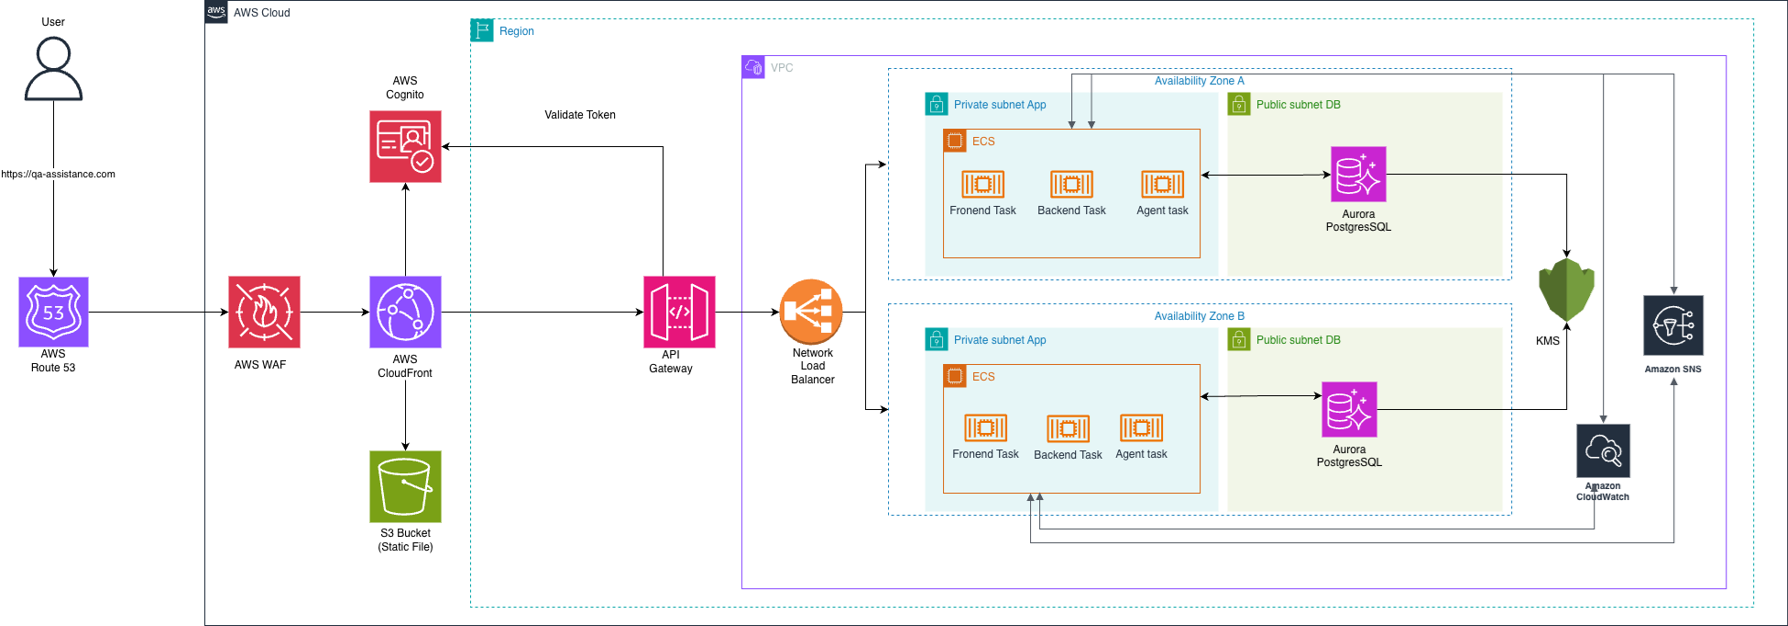
\includegraphics[width=0.98\textwidth,height=0.42\textheight,keepaspectratio]{SystemArchitecture.png}
\caption{Proposed AWS deployment architecture for the Quality Assistance application. This target design is not currently deployed by the repository.}
\label{fig:system-architecture-deployment}
\end{figure}

\subsection{Frontend}
The frontend covers sign-in, a dashboard for assistance requests, settings, and a short user guide. On the dashboard a user can type free-form requirements and stories, paste a code change, and start from sample requests: smoke planning, an end-to-end example, change impact, execution and reporting, automation, and a follow-up turn. If Jira is connected, assigned issues can fill the story field. If GitHub is connected, a pull-request or compare diff can be fetched rather than pasted. The reply is shown in the browser and can be downloaded as Markdown or HTML.

\subsection{Backend and Persistence}
The backend is a FastAPI service using asynchronous SQLAlchemy against PostgreSQL \cite{fastapidocs}. The \texttt{/api/assist} route is authenticated. It stores a request with its owner, source text, session identifier, status, timestamps, and, later, the response. It then builds a structured agent message and calls the agent service. Success and failure are both recorded. Errors go back to the frontend through the API's usual error path.

Users, assistance requests, Jira connections, and GitHub repository connections are stored as separate records. That is enough to look up an earlier submission. It is not enough to treat agent conversations as durable history. The current ADK runner keeps session state in memory, so a restart can drop a follow-up context that a user still has on screen.

\subsection{Agent Orchestration}
The root agent is named \texttt{quality\_assistance\_agent}. It is assembled with Google ADK, a configured model, logging callbacks, and the tools that are available at start-up \cite{googleadk}. For the supported cloud providers the root agent can hand work to registered sub-agents. The local Ollama path uses a single, consolidated instruction instead; the specialists are not transferred in that configuration. The backend prompt asks for prioritized test cases, suggested data, automation notes, and release risks, built from the requirements, stories, and diffs that were submitted.

\begin{table}[htbp]
\centering
\small
\begin{tabularx}{\textwidth}{p{0.06\textwidth}p{0.34\textwidth}X}
\toprule
\textbf{ID} & \textbf{Specialist} & \textbf{Implemented responsibility} \\
\midrule
S01 & Test case generation & Drafts structured, prioritized cases from requirements and stories, including positive, negative, and boundary scenarios. \\
S02 & Test data generation & Suggests representative and edge-case test data. \\
S03 & Test script automation & Suggests automation approaches and repeatable script outlines. \\
S04 & Test execution & Interprets supplied or simulated test-run results and highlights failures; it does not itself launch the user's test suite. \\
S05 & Self-healing test scripts & Recommends maintenance strategies when selectors or interfaces change; it does not directly edit repository files. \\
S06 & Change impact analysis & Relates supplied code diffs to potentially affected areas and regression scope. \\
S07 & Bug report generation & Structures failure information into an actionable defect report. \\
S08 & Test summary reporting & Summarizes test outcomes for stakeholders. \\
S09 & Release readiness evaluation & Weighs supplied test and risk signals and provides a reasoned recommendation. \\
\bottomrule
\end{tabularx}
\caption{Registered specialist agents and the scope described by their instructions.}
\label{tab:agents}
\end{table}

The router maps requirement and story text to the test-case and test-data agents, diffs to change-impact analysis, execution logs to the execution, defect, and summary agents, and release questions to readiness. There is also a requirement-summarization tool on the root agent. This is prompt-driven routing. There is no separate deterministic workflow engine sitting beside it.

\begin{figure}[H]
\centering
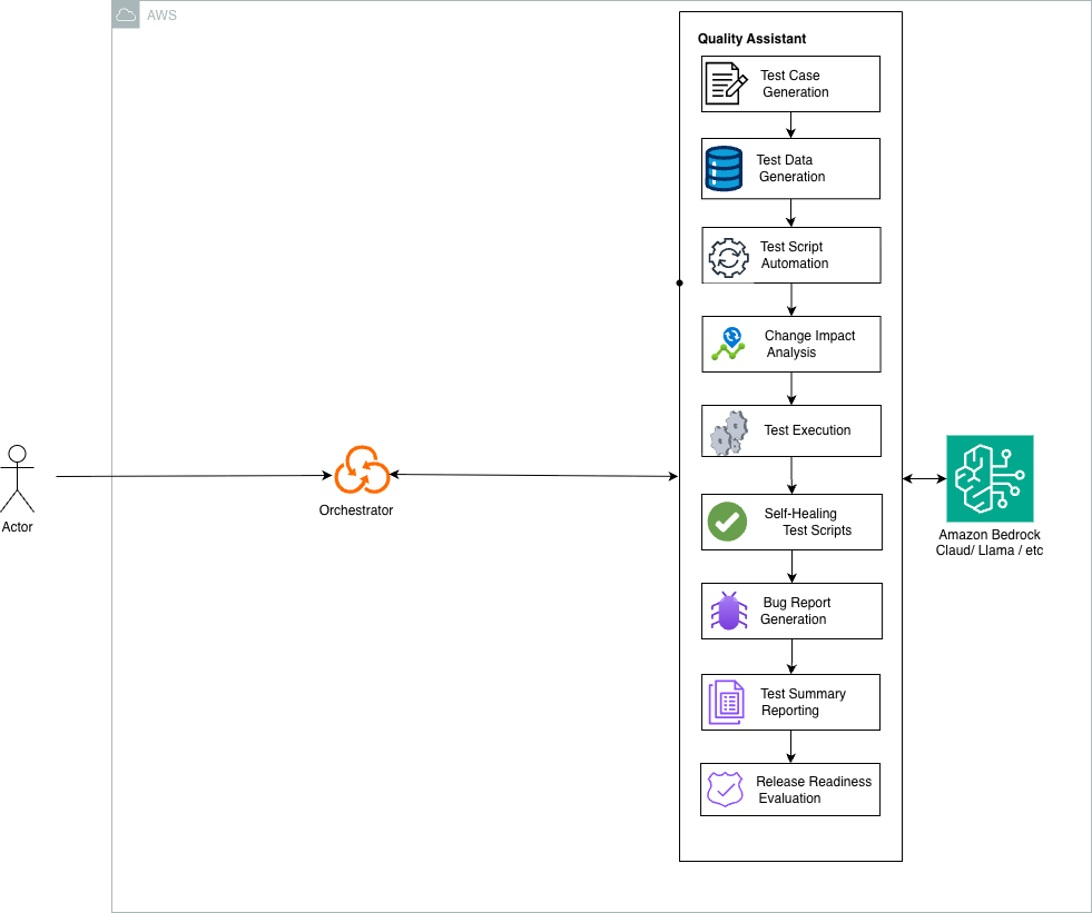
\includegraphics[width=0.72\textwidth,height=0.45\textheight,keepaspectratio]{agentic_flow.jpg}
\caption{Illustrative agentic workflow showing orchestration among the root agent and specialist agents.}
\label{fig:agentic-flow}
\end{figure}

\begin{algorithm}[htbp]
\caption{Assistance request processing}
\label{alg:assistance}
\begin{algorithmic}[1]
\Require Authenticated user $u$, requirements $r$, optional stories $s$, diff $d$, session $q$
\State Validate the request and associate it with $u$
\State Persist request inputs with status \texttt{processing}
\State Construct a message from $r$, $s$, and $d$
\State Resolve or create an agent session for $u$
\State Invoke the root agent with the message and session
\State Route to one or more specialists according to the request context
\State Collect the generated response from the agent events
\If{agent call succeeds}
  \State Persist session identifier, response, and status \texttt{completed}
\Else
  \State Persist failure status and return an explicit service error
\EndIf
\State Return the request identifier, session, response, and status
\end{algorithmic}
\end{algorithm}

\begin{figure}[H]
\centering
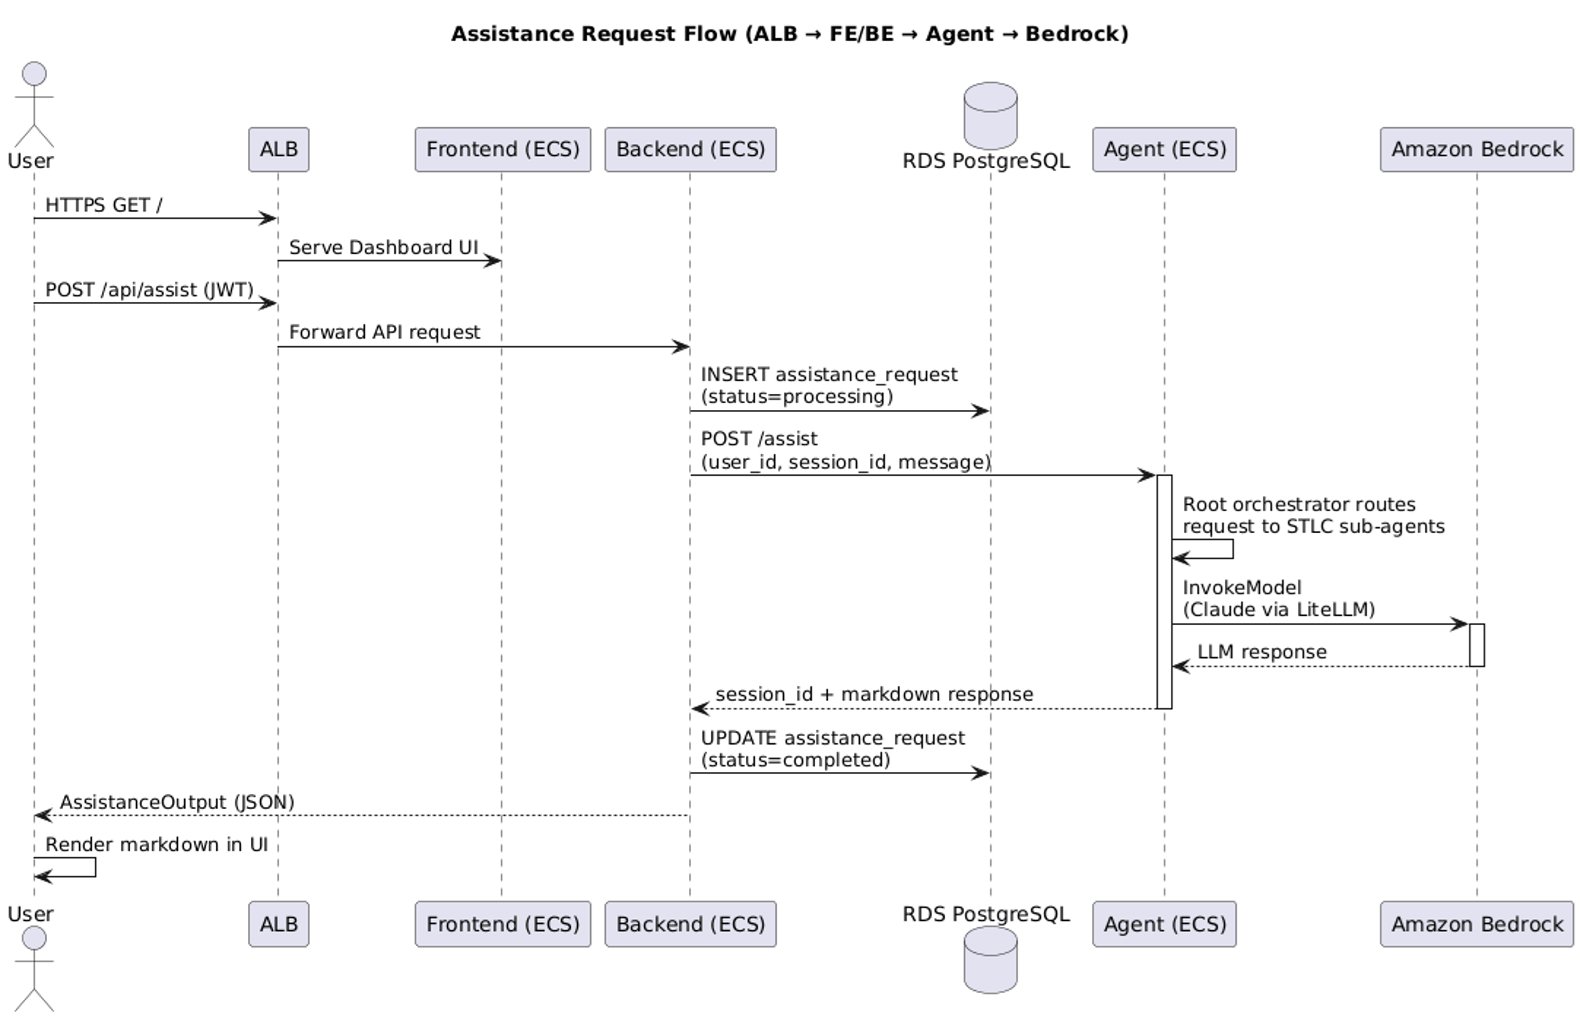
\includegraphics[width=0.92\textwidth,height=0.48\textheight,keepaspectratio]{sequence_daigram.png}
\caption{Illustrative request sequence through the application services for the deployment configuration shown.}
\label{fig:request-sequence}
\end{figure}

\subsection{External Integrations and Model Providers}
Jira Cloud uses OAuth 2.0, a short-lived state record, and Jira APIs to list a user's assigned issues and to fetch issue detail. GitHub settings store a repository and an encrypted personal access token; the backend can then pull a pull-request diff or compare two references. Microsoft Entra single sign-on is optional. The agent configuration accepts Gemini, LiteLLM, Amazon Bedrock, and Ollama, provided credentials and models are available. Those are options in the code. They are not a claim that every provider was benchmarked on the same tasks.

\section{Security and Data Handling}
Assistance records belong to the signed-in user. JWT access tokens are issued after registration or login. Password handling is delegated to the project's password manager. Jira and GitHub credentials are stored encrypted. Jira OAuth state is a digest and it expires. In production the settings check looks for real secrets, an encryption key, explicit HTTPS origins, database TLS, and non-default database credentials. The ECS guide describes a pattern with private application and database services, IAM roles, and managed secrets.

Requirements, stories, diffs, and test results can easily contain proprietary information. The application stores them with the request and sends them to whatever model provider is configured. Anyone deploying this has to pick a provider and retention policy that their organization will accept, restrict who can see stored data, rotate credentials, and keep secrets out of the prompt. The controls in the prototype reduce accidental exposure. They do not replace a privacy assessment, a threat model, an independent review, or an internal approval.

\section{Deployment and Operations}
For local work the repository has a Docker Compose stack covering PostgreSQL, frontend, backend, and agent. There are also scripts for a local frontend and Python services against a local or containerized database. The AWS ECS Fargate notes describe a pilot with separate containers, RDS PostgreSQL, an Application Load Balancer, and a chosen model provider. That document is a checklist. It is not infrastructure-as-code, and this report does not claim that an AWS production environment has been stood up.

\section{Quality Attributes}
\begin{itemize}
  \item \textbf{Modularity:} frontend, API, persistence, and agent service are separate processes; specialists are registered on their own.
  \item \textbf{Configurability:} model providers, endpoints, integrations, and production flags come from the environment.
  \item \textbf{Traceability:} the backend stores each user's inputs and responses; a formal requirement-to-case evidence trail and durable agent memory are still missing.
  \item \textbf{Availability:} health and readiness endpoints and container notes help operations; how resilient a real deployment is depends on the topology that is actually chosen.
  \item \textbf{Reliability:} the backend has explicit error paths and settings checks. Generated quality artifacts still need a person to read them, and they still need an empirical evaluation.
\end{itemize}

\chapter{Results and Discussions}
\label{chap:experiments_and_results}

\section{Prototype Implementation Status}
The repository contains a working full-stack prototype, not just an architecture proposal. A user can register and sign in, submit context through an authenticated API, and review a response in the dashboard. Requests are persisted, and the separate agent service registers nine specialists that the root agent can select through its routing instructions. The source also includes GitHub diff retrieval, Jira Cloud OAuth and issue retrieval, and optional Microsoft Entra authentication.

\begin{table}[htbp]
\centering
\small
\begin{tabularx}{\textwidth}{p{0.30\textwidth}p{0.20\textwidth}X}
\toprule
\textbf{Project area} & \textbf{Status in inspected repository} & \textbf{Evidence or qualification} \\
\midrule
Problem analysis and architecture & Implemented & Research framing is documented in the proposal and presentation; current services are separated into frontend, backend, and agent. \\
Core quality-assistance flow & Implemented & Authenticated request persistence, prompt construction, agent call, and response persistence are present. \\
Specialist STLC capabilities & Implemented & Nine task-focused agents are registered; orchestration is controlled by ADK and agent instructions. \\
Jira and GitHub context & Implemented, configuration-dependent & OAuth and issue retrieval are available for Jira; GitHub repository settings support diff retrieval. \\
Authentication and deployment controls & Implemented in part & Password/JWT authentication, optional Entra SSO, encrypted integration credentials, and production settings validation are present. \\
RAG over organizational test assets & Planned & No persistent requirements/test/defect retrieval index is evidenced in the inspected implementation. \\
Automated CI test execution and script mutation & Planned / out of scope of current behavior & Execution and healing agents analyze or recommend; they do not execute external suites or commit changes. \\
Comparative empirical evaluation & Pending & No measured baseline, benchmark results, or controlled organizational pilot results were supplied. \\
\bottomrule
\end{tabularx}
\caption{Implementation status as of November 2026, distinguishing current behavior from planned work.}
\label{tab:implementation-status}
\end{table}

\section{Existing Automated Test Assets}
Focused test modules cover Bedrock credential settings, backend production configuration, Jira Cloud service behavior, and Microsoft Entra SSO behavior. These tests show that selected configuration and integration paths have dedicated checks. They do not establish that the tests pass, nor do they validate every UI, model, database, or agent workflow end to end. A reproducible submission should include the command, environment, commit, test count, and outcome from an actual run.

\section{Demonstration Scenarios}
The dashboard includes sample inputs that can be used to demonstrate several agent routes:
\begin{enumerate}
  \item a password-reset requirement for test planning and requirement summarization;
  \item an e-commerce checkout scenario with requirements, user stories, and a code diff;
  \item a diff-heavy authentication change for regression impact analysis;
  \item a test-run log containing pass, fail, and skipped cases for execution analysis and reporting;
  \item a Playwright selector change for automation and self-healing recommendations; and
  \item a follow-up request that reuses the prior session identifier.
\end{enumerate}
These examples show that the interface and request model can handle several kinds of context. They are demonstrations, not a benchmark, and provide no measurement of coverage, effort, or defect detection.

\subsection{Interface Walkthrough and Illustrative Outputs}
The screenshots follow a typical request: opening the workspace, checking integration settings, entering requirements and a user story, then reviewing the response. They document the interface and sample output only. No controlled evaluation was performed, and recommendations shown here still need human review.

\begin{figure}[H]
\centering
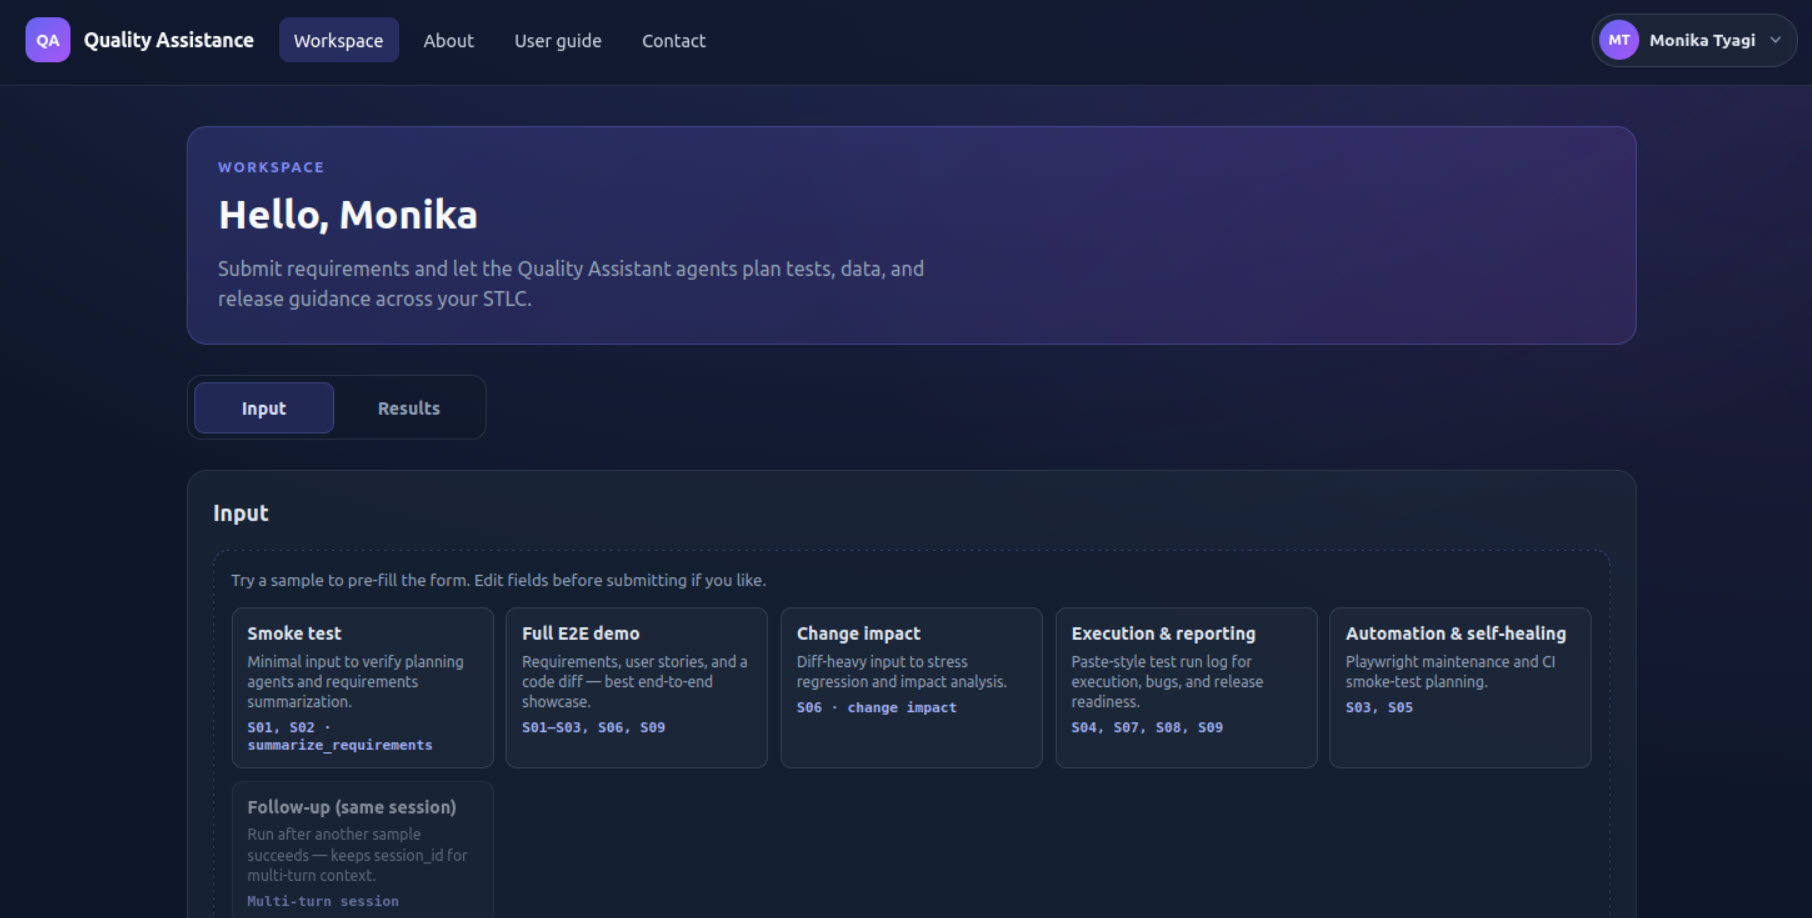
\includegraphics[width=\textwidth,height=0.46\textheight,keepaspectratio]{home.jpg}
\caption{Workspace dashboard used to start a quality-assistance request.}
\label{fig:workspace-dashboard}
\end{figure}

\begin{figure}[H]
\centering
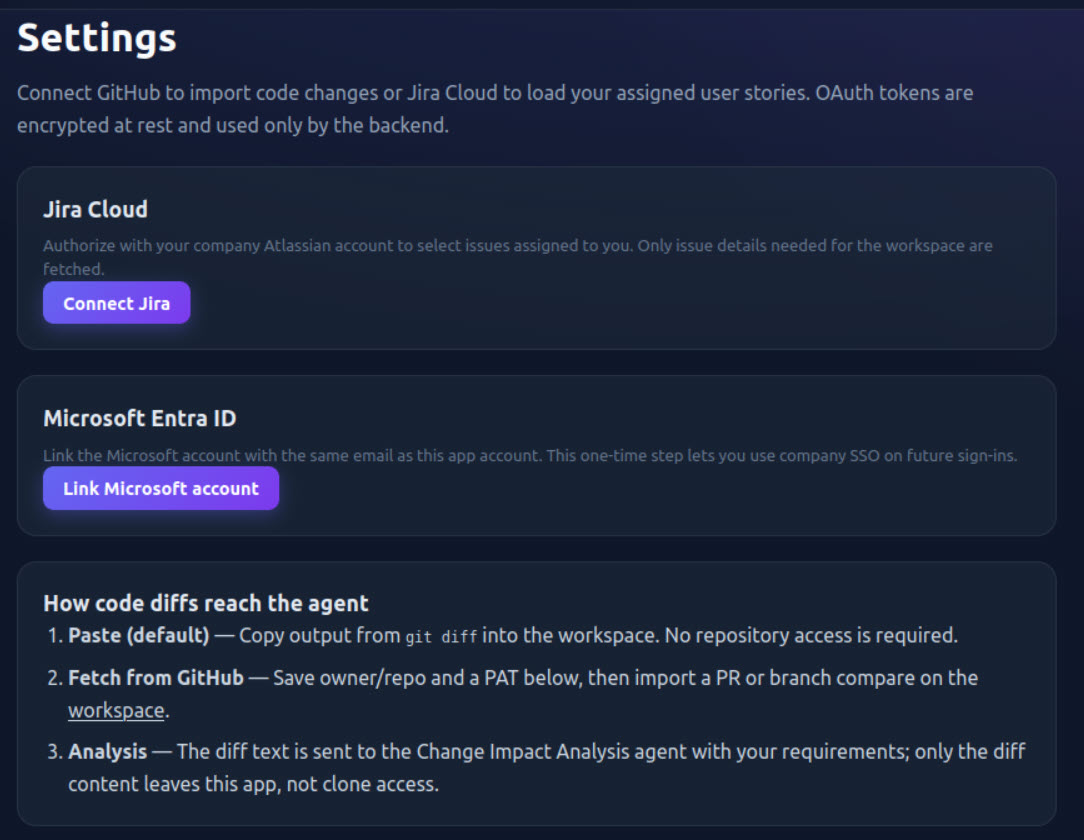
\includegraphics[width=0.9\textwidth,height=0.46\textheight,keepaspectratio]{settings.jpg}
\caption{Settings page for configuring Jira, GitHub, and sign-in integrations. Availability depends on administrator configuration and valid credentials.}
\label{fig:integration-settings}
\end{figure}

\begin{figure}[H]
\centering
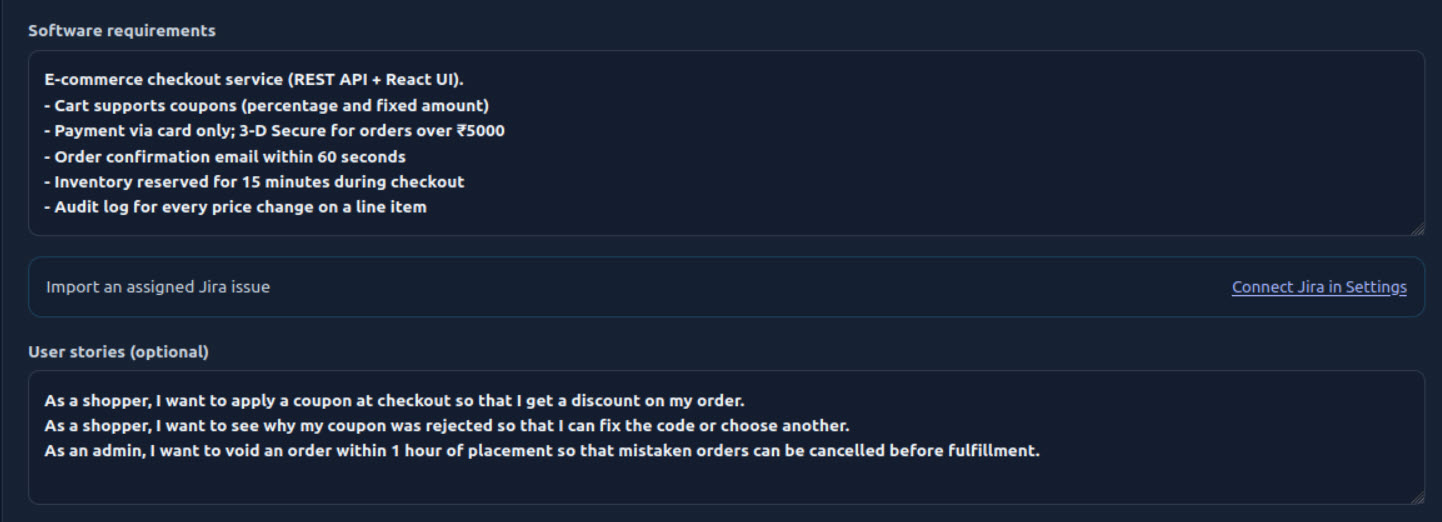
\includegraphics[width=\textwidth,height=0.42\textheight,keepaspectratio]{input.jpg}
\caption{Example request input containing quality context and a user story before agent processing.}
\label{fig:request-input}
\end{figure}

\begin{figure}[H]
\centering
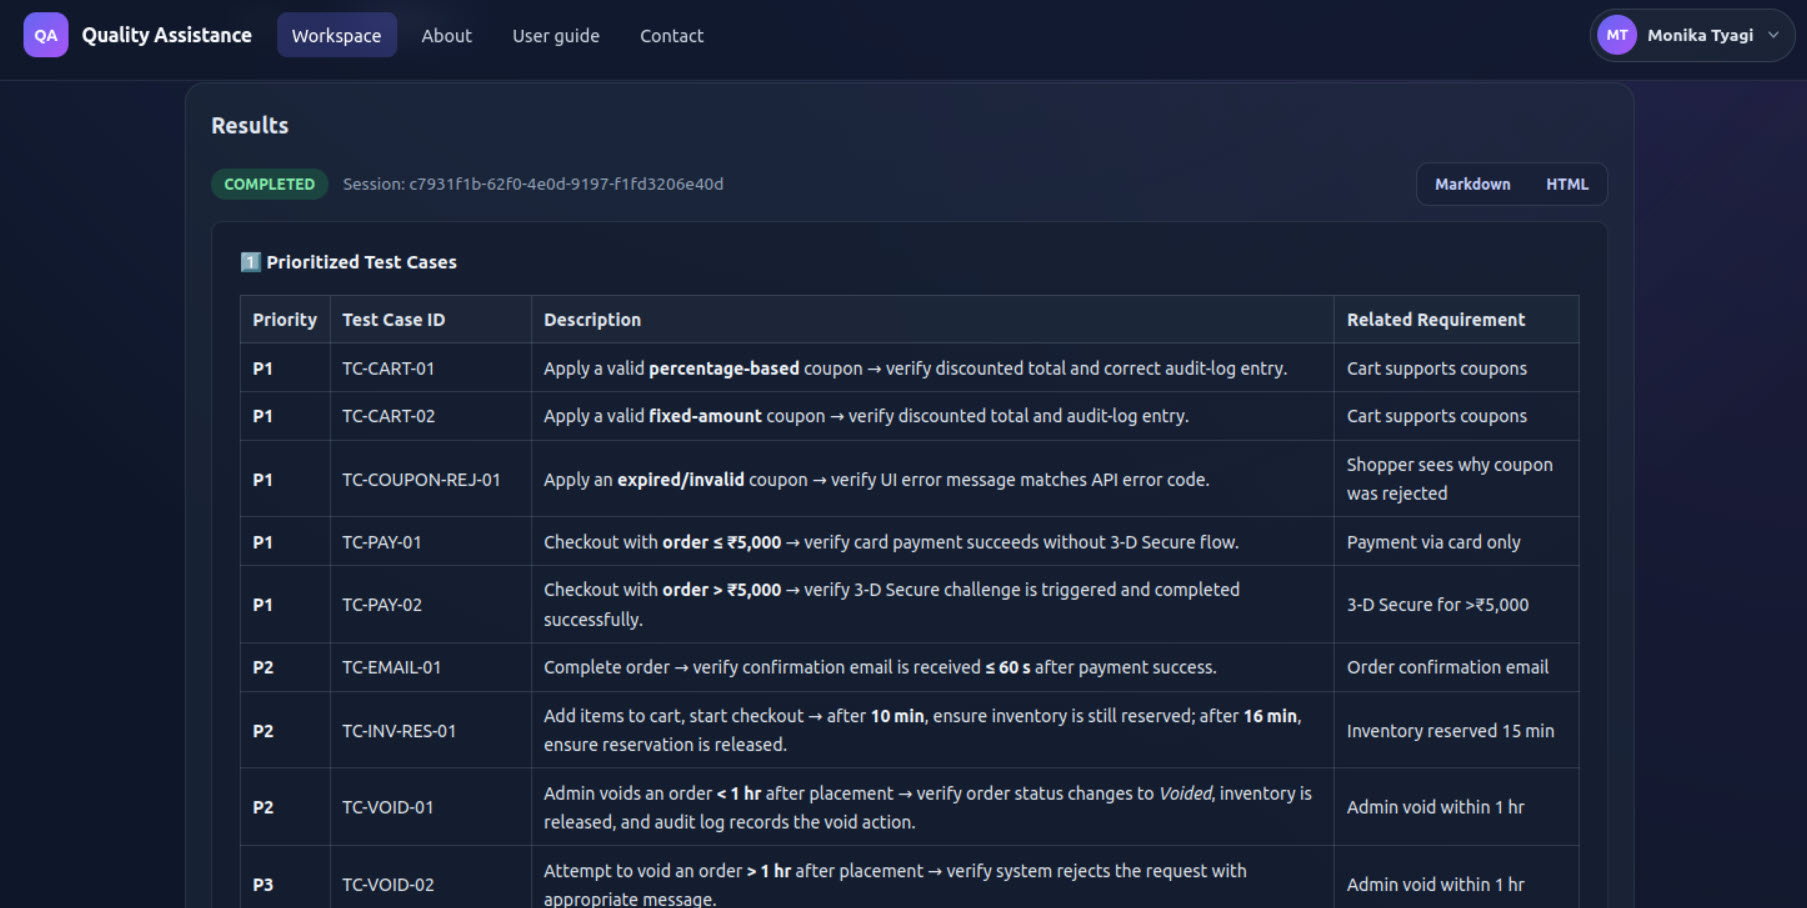
\includegraphics[width=\textwidth,height=0.46\textheight,keepaspectratio]{result.jpg}
\caption{Example generated response with prioritized test-case recommendations.}
\label{fig:prioritized-results}
\end{figure}

\begin{figure}[H]
\centering
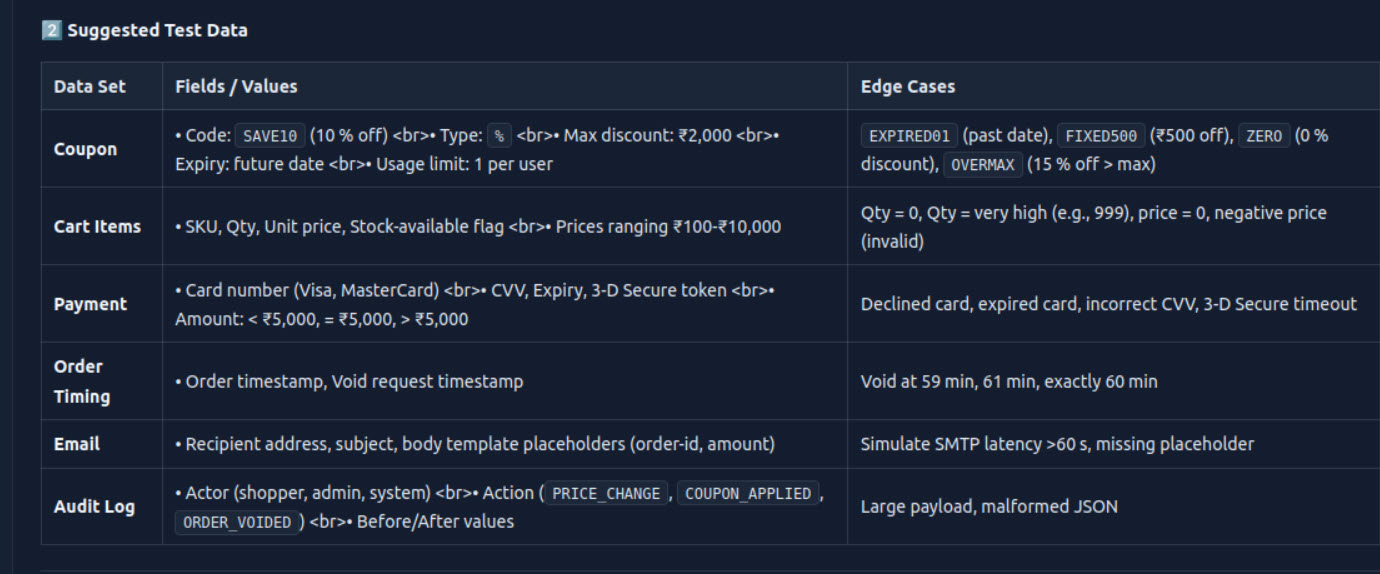
\includegraphics[width=\textwidth,height=0.42\textheight,keepaspectratio]{result2.jpg}
\caption{Example suggested test data presented as part of the generated response.}
\label{fig:suggested-test-data}
\end{figure}

\begin{figure}[H]
\centering
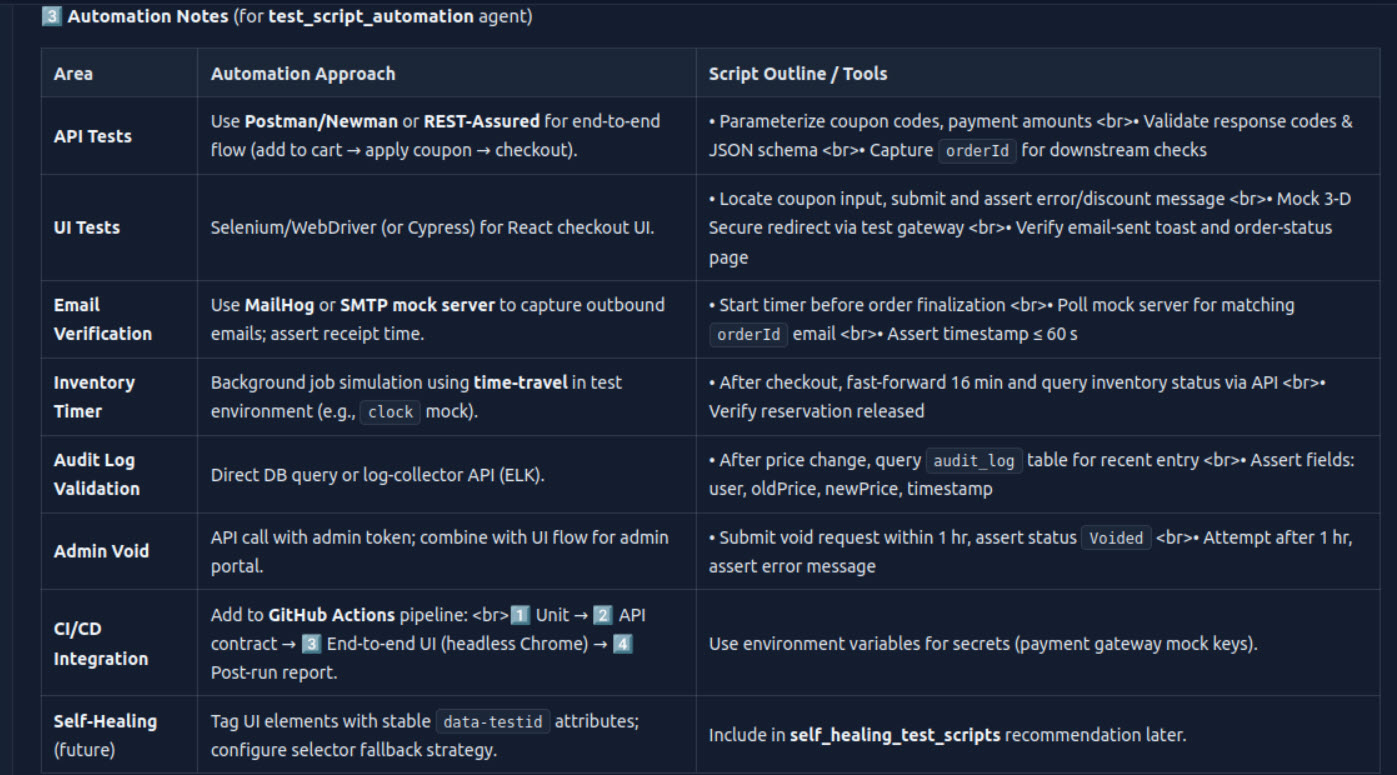
\includegraphics[width=\textwidth,height=0.46\textheight,keepaspectratio]{result3.jpg}
\caption{Example automation notes and test-script recommendations.}
\label{fig:automation-results}
\end{figure}

\begin{figure}[H]
\centering
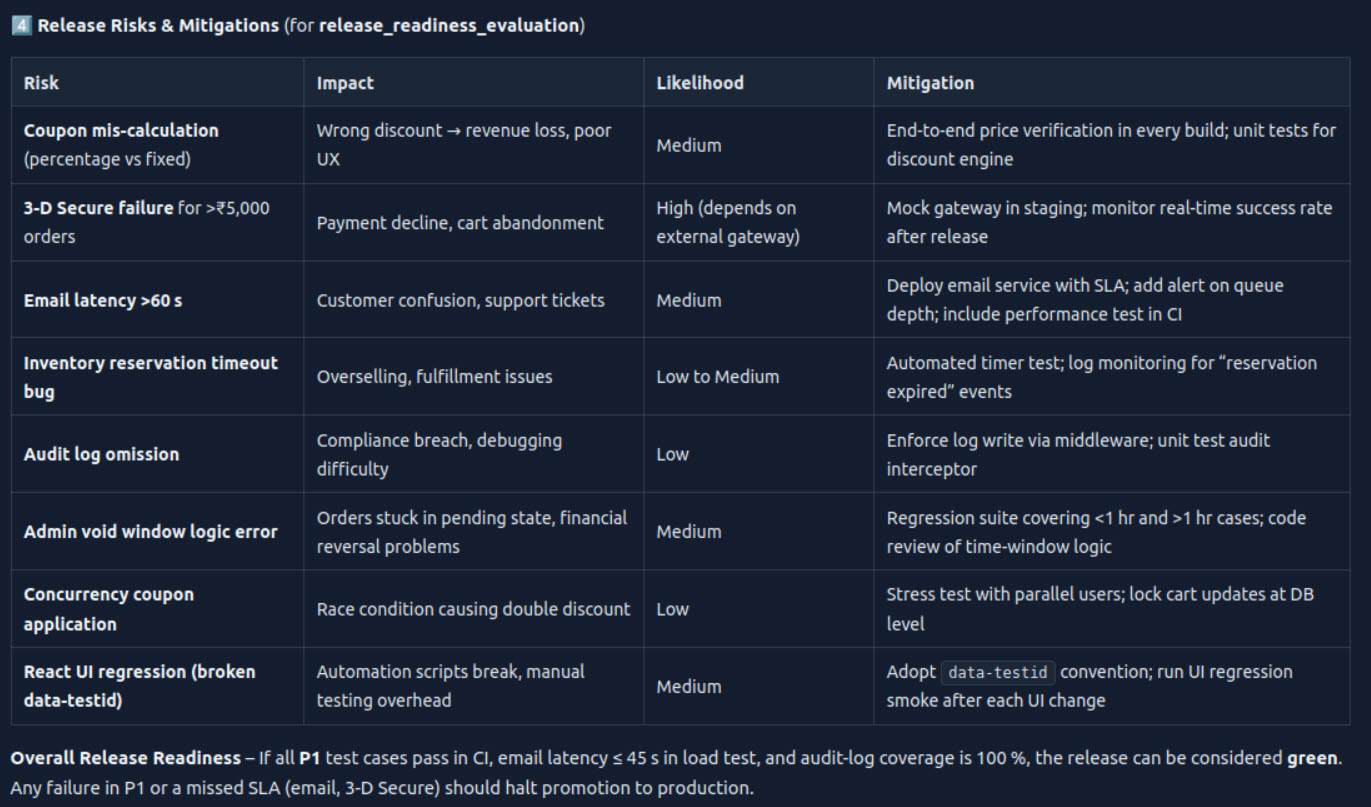
\includegraphics[width=\textwidth,height=0.46\textheight,keepaspectratio]{result4.jpg}
\caption{Example release-risk and readiness analysis based on the submitted context.}
\label{fig:readiness-results}
\end{figure}

\section{Evaluation Plan}
The evaluation should compare three conditions on the same tasks: a manual QA baseline, an existing point-automation workflow where available, and the proposed assistant-supported workflow. The initial phase should use public requirements and open-source repositories or issue trackers, as proposed in the project plan. Any later organizational evaluation should use anonymized artifacts and receive the required data-governance approval.

\subsection{Dataset and Protocol}
For each project, select a bounded set of requirements, user stories, code changes, and available test-run or defect records. Define expected requirement-to-test links and expert-reviewed reference outputs before running the assistant. Use a fixed model, model version, prompt revision, and application configuration for each comparison. Because model outputs can vary, repeat tasks where practical and retain both raw outputs and review decisions. The reviewer should be blind to the workflow condition when rating generated artifacts, where feasible.

\subsection{Measures}
\begin{table}[htbp]
\centering
\small
\begin{tabularx}{\textwidth}{p{0.25\textwidth}p{0.31\textwidth}X}
\toprule
\textbf{Measure} & \textbf{Operational definition} & \textbf{Interpretation} \\
\midrule
Requirement traceability & Percentage of in-scope requirements linked to at least one reviewer-accepted test case. & Tests whether generated artifacts preserve requirement coverage links. \\
Scenario coverage & Reviewer-rated coverage of agreed positive, negative, boundary, and risk conditions. & Measures breadth and relevance rather than the raw number of generated cases. \\
Artifact correctness & Proportion of sampled cases judged correct and actionable by independent reviewers. & Captures factual and procedural quality; report agreement between reviewers. \\
Effort & Active authoring and review time per requirement or change. & A reduction is meaningful only if review and correction time are included. \\
Defect analysis quality & Precision, recall, or F-score against adjudicated defect categories when labels exist. & Applies only where a suitable labeled reference set is available. \\
Response time and cost & End-to-end latency and model usage per completed task. & Quantifies operational overhead and helps assess scalability. \\
User acceptance & Structured ratings of usefulness, clarity, and trust from representative practitioners. & Complements objective measures but should not replace correctness review. \\
\bottomrule
\end{tabularx}
\caption{Proposed evaluation measures; no values are reported because a controlled evaluation has not yet been completed.}
\label{tab:evaluation-metrics}
\end{table}

\subsection{Analysis and Validity}
For quantitative comparisons, report sample sizes, distributions, confidence intervals, and the selected statistical tests. Analyze error categories as well as aggregate scores. Conduct qualitative review of omissions, unsupported statements, ambiguous requirements, and cases where the model's recommendation conflicts with expert judgment. Record the model and prompt versions so that repeated evaluations remain interpretable.

Threats to validity include dataset representativeness, evaluator subjectivity, model nondeterminism, changes in external model services, contamination between task examples and prompts, and the possibility that generated cases increase review burden. A small public-data evaluation would support feasibility claims but would not alone establish generalization to enterprise workflows.

\section{Results and Discussion}
The evidence available here is implementation evidence. The application accepts quality context, stores a request, calls the orchestrated agent, and returns a response. Its specialist registry and dashboard examples cover several STLC tasks, while the integration code provides a starting point for connecting engineering systems.

The materials reviewed for this report did not include experiment results, a benchmark dataset, measured time savings, coverage figures, defect-detection rates, or user-study findings. It is therefore not possible to claim that the system improves quality or reduces effort. The result at this stage is the software artifact and a protocol for testing those claims. Plausible-looking generated cases are not, on their own, evidence that the cases are complete, correct, or effective at finding defects.

\section{Limitations}
\begin{itemize}
  \item The quality of recommendations depends on the completeness and accuracy of user-supplied context and the selected model.
  \item Cross-agent routing and synthesis are predominantly prompt-driven; formal inter-stage schemas and independent quality gates are not evidenced.
  \item Agent session state uses an in-memory runner and is not a durable conversation store across process restarts.
  \item The system does not autonomously execute external test suites, modify scripts, or enforce release approvals.
  \item Persistent retrieval over requirements, test assets, and historical defects and a Jenkins or equivalent CI/CD integration are future work.
  \item The available repository tests address selected settings and service behavior; comprehensive user-interface, model-quality, load, and end-to-end tests remain necessary.
  \item Production deployment and organization-specific security and privacy approval are not demonstrated by the deployment planning documents.
\end{itemize}

\chapter{Conclusions}
\label{chap:conclusion}

The aim was to keep several STLC jobs in one place. The repo now has a full-stack application that does that, at least as a draft workflow. The React and TypeScript UI, the FastAPI and PostgreSQL backend, and the Google ADK agent service meet at a root agent that can send work to nine specialists. Those specialists write test design and data, comment on a change, draft a defect, and write release-readiness notes. Login, request storage, Jira Cloud and GitHub context, optional Microsoft Entra SSO, and a choice of model providers are also there.

Getting those pieces to talk to each other was the engineering work. It is not the same as showing that quality improved. I have not run a controlled comparison, so I cannot say the assistant improves coverage, cuts the time a tester spends, or finds more defects. The agents write drafts. Someone still has to judge them. Execution analysis does not launch a suite. A self-healing note does not change the code. A readiness paragraph does not approve a release.

\section{Future Work}
What I would do next, in order:
\begin{enumerate}
  \item structured outputs and checks between specialist stages;
  \item a place for a person to approve or edit test cases, and anything that could affect a release;
  \item an evaluation of traceability, correctness, review effort, latency, and cost against a baseline written down in advance;
  \item trials on public projects and, after approval, on anonymized organisational artifacts;
  \item retrieval over approved requirements, test repos, and historical defects;
  \item a careful CI/CD hook for test execution, and session history that survives a restart and can be audited; and
  \item load, reliability, accessibility, privacy, and security reviews before this is treated as a wider deployment.
\end{enumerate}

I already know an LLM can write something that looks like a test case. The question I still cannot answer is whether this orchestrated assistant produces work that people can trace and use, often enough that the review it creates is still cheaper than doing the task without it. The prototype is the place to run that comparison. Screenshots of a working demo are not the comparison.


\backmatter
\bibliographystyle{unsrtnat}
\renewcommand{\bibname}{References}
\bibliography{references}
\end{document}
